\begin{align*}
    \polynomialQ{3}{X}{0} &= 0 \\
    \polynomialQ{3}{X}{1} &= 1 \\
    \polynomialQ{3}{X}{2} &= 140X^3 - 420X^2 + 406X - 124 \\
    \polynomialQ{3}{X}{3} &= 1260X^3 - 7140X^2 + 13818X - 9027 \\
    \polynomialQ{3}{X}{4} &= 5040X^3 - 41160X^2 + 115836X - 110960 \\
    \polynomialQ{3}{X}{5} &= 14000X^3 - 148680X^2 + 545860X - 684175 \\
    \polynomialQ{3}{X}{6} &= 31500X^3 - 411180X^2 + 1858290X - 2871324 \\
    \polynomialQ{3}{X}{7} &= 61740X^3 - 955500X^2 + 5124126X - 9402659 \\
    \polynomialQ{3}{X}{8} &= 109760X^3 - 1963920X^2 + 12182968X - 25872832 \\
    \polynomialQ{3}{X}{9} &= 181440X^3 - 3684240X^2 + 25945416X - 62572095 \\
    \polynomialQ{3}{X}{10} &= 283500X^3 - 6439860X^2 + 50745870X - 136972700 \\
    \polynomialQ{3}{X}{11} &= 423500X^3 - 10639860X^2 + 92745730X - 276971299 \\
    \polynomialQ{3}{X}{12} &= 609840X^3 - 16789080X^2 + 160386996X - 524988144 \\
    \polynomialQ{3}{X}{13} &= 851760X^3 - 25498200X^2 + 264896268X - 943023887 \\
    \polynomialQ{3}{X}{14} &= 1159340X^3 - 37493820X^2 + 420839146X - 1618774780 \\
    \polynomialQ{3}{X}{15} &= 1543500X^3 - 53628540X^2 + 646725030X - 2672907075 \\
    \polynomialQ{3}{X}{16} &= 2016000X^3 - 74891040X^2 + 965662320X - 4267591424 \\
    \polynomialQ{3}{X}{17} &= 2589440X^3 - 102416160X^2 + 1406064016X - 6616398079 \\
    \polynomialQ{3}{X}{18} &= 3277260X^3 - 137494980X^2 + 2002403718X - 9995653692 \\
    \polynomialQ{3}{X}{19} &= 4093740X^3 - 181584900X^2 + 2796022026X - 14757360515 \\
    \polynomialQ{3}{X}{20} &= 5054000X^3 - 236319720X^2 + 3835983340X - 21343778800
\end{align*}
\begin{figure}[H]
    \centering
    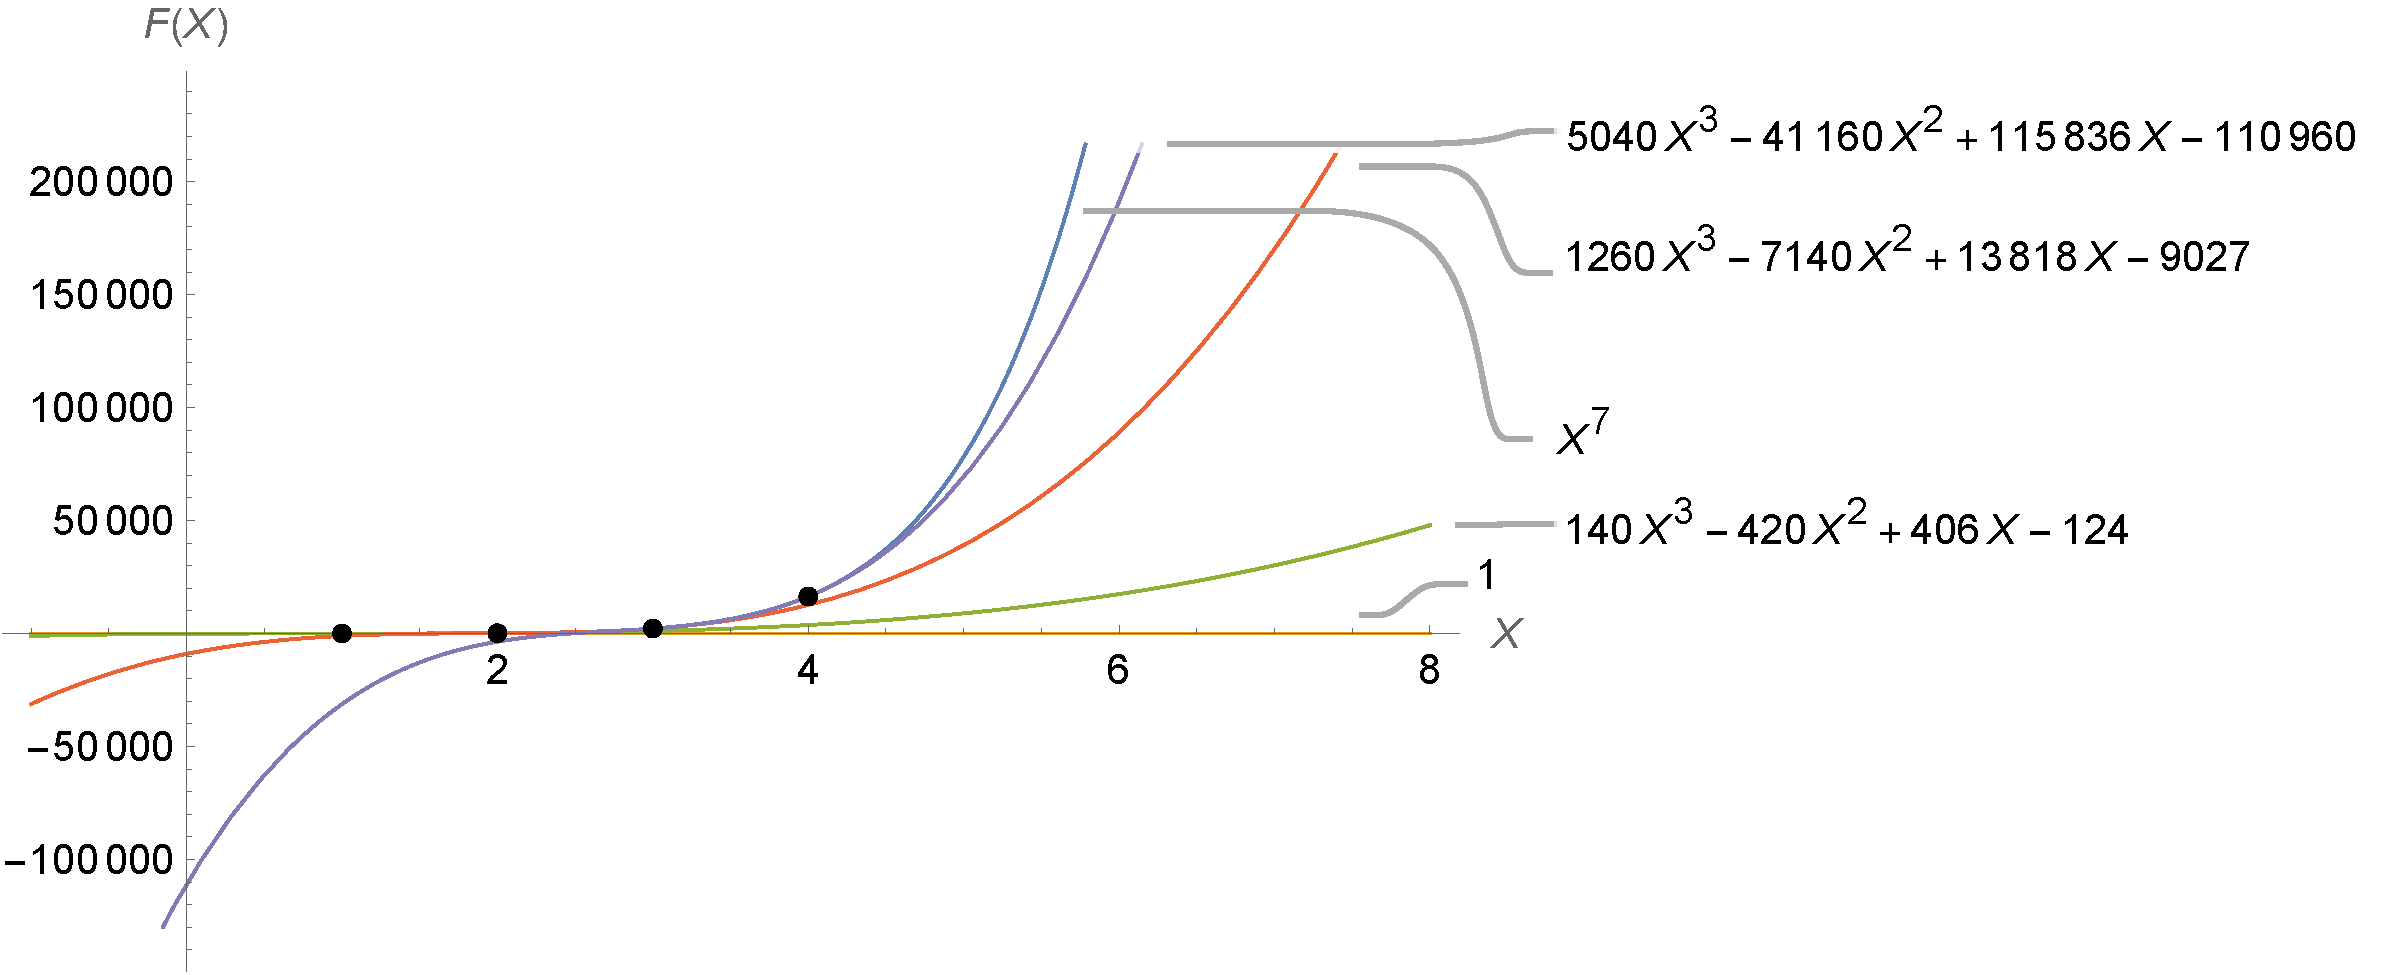
\includegraphics[width=1\textwidth]{sections/images/06_seventh_power_with_q_3_n_k}
    ~\caption{Polynomials P(1, n, k)}\label{fig:figure6}
\end{figure}
